
CMake is a cross-platform, open-source software written in C++. That means you can, of course, compile it yourself; however, the most likely scenario is that you won't have to. This is because precompiled binaries are available for you to download from the official web page at \url{https://cmake.org/download/}.

Unix-based systems provide ready-to-install packages directly from the command line..

\begin{tcolorbox}[colback=blue!5!white,colframe=blue!75!black,title=Note]
Remember that CMake doesn't come with compilers. If your system doesn't have them installed yet, you'll need to provide them before using CMake. Make sure to add the paths to their executables to the PATH environment variable so that CMake can find them.

To avoid solving tooling and dependency problems while learning from this book, I recommend choosing the first installation method: Docker.
\end{tcolorbox}

Let's go through different environments on which CMake can be used.

\subsubsubsection{1.3.1\hspace{0.2cm}Docker}

Docker (\url{https://www.docker.com/}) is a cross-platform tool that provides OS-level virtualization, allowing applications to be shipped in complete packages, called containers. These are self-sufficient bundles that contain a piece of software with all of its libraries, dependencies, and tools required to run it. Docker executes its containers in lightweight environments that are isolated one from another.

This concept makes it extremely convenient to share whole toolchains, which are necessary for a given process, configured and ready to go. I can't stress enough how easy things become when you don't need to worry about minuscule environmental differences. 

The Docker platform has a public repository of container images, \url{https://registry.hub.docker.com/}, that provides millions of ready-to-use images.

For your convenience, I have published two Docker repositories:

\begin{itemize}
\item 
swidzinski/cmake:toolchain: This contains the curated tools and dependencies that are necessary to build with CMake.

\item 
swidzinski/cmake:examples: This contains the preceding toolchain and all of the projects and examples from this book.
\end{itemize}

The first option is for readers who simply want a clean-slate image ready to build their own projects, and the second option is for hands-on practice with examples as we go through the chapters.

You can install Docker by following the instructions from its official documentation (please refer to \url{docs.docker.com/get-docker}). Then, execute the following commands in your Terminal to download the image and start the container:

\begin{tcblisting}{commandshell={}}
$ docker pull swidzinski/cmake:examples
$ docker run -it swidzinski/cmake:examples
root@b55e271a85b2:root@b55e271a85b2:#
\end{tcblisting}

Note that all of the examples are available in the directories matching this format: \texttt{/root/examples/examples/chapter-<N>/<M>-<title>}.

\subsubsubsection{1.3.2\hspace{0.2cm}Windows}

Installing in Windows is straightforward – simply download the version for 32 or 64 bits. You can pick a portable ZIP or MSI package for Windows Installer.

With the ZIP package, you will have to add the CMake bin directory to the PATH environment variable so that you can use it in any directory without any such errors:

\begin{tcblisting}{commandshell={}}
'cmake' is not recognized as an internal or external command,
operable program or batch file.
\end{tcblisting}

If you prefer convenience, simply use the MSI installer:

\begin{center}
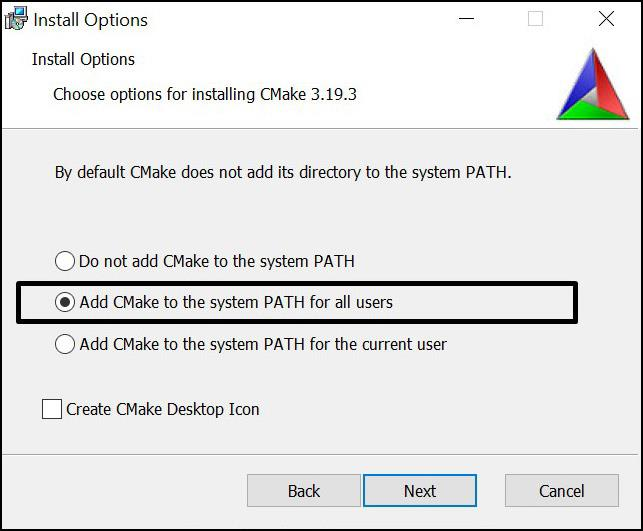
\includegraphics[width=0.9\textwidth]{content/1/chapter1/images/2.jpg}\\
Figure 1.2 – The installation wizard can set up the PATH environment variable for you
\end{center}

As I mentioned earlier, this is open-source software, so it is possible to build CMake yourself. However, first, you will have to get a binary copy of CMake on your system. So, why use other build tools if you have your own, right? This scenario is used by CMake contributors to generate newer versions.

On Windows, we also require a build tool that can finalize the build process started by  CMake. A popular choice here is Visual Studio, for which the Community Edition is available for free from Microsoft's website: \url{https://visualstudio.microsoft.com/downloads/}.

\subsubsubsection{1.3.3\hspace{0.2cm}Linux}

Getting CMake on Linux is the same as getting any other popular package. Simply use your package manager from the command line. Packages are usually kept up to date with fairly recent versions. However, if you are after the latest version, you can download the installation script from the website:

\hspace*{\fill} \\ %插入空行
\noindent
\textbf{The script for Linux x86\_64}

\begin{tcblisting}{commandshell={}}
$ wget -O - https://github.com/Kitware/CMake/releases/download/
v3.20.0/cmake-3.20.0-linux-x86_64.sh | bash
\end{tcblisting}

\hspace*{\fill} \\ %插入空行
\noindent
\textbf{The script for Linux aarch64}

\begin{tcblisting}{commandshell={}}
$ wget -O - https://github.com/Kitware/CMake/releases/download/
v3.20.0/cmake-3.20.0-Linux-aarch64.sh | bash
\end{tcblisting}

\hspace*{\fill} \\ %插入空行
\noindent
\textbf{The package for Debian/Ubuntu}

\begin{tcblisting}{commandshell={}}
$ sudo apt-get install cmake
\end{tcblisting}

\hspace*{\fill} \\ %插入空行
\noindent
\textbf{The package for Red Hat}

\begin{tcblisting}{commandshell={}}
$ yum install cmake
\end{tcblisting}

\subsubsubsection{1.3.4\hspace{0.2cm}macOS}

This platform is also strongly supported by CMake developers. The most popular choice of installation is through MacPorts:

\begin{tcblisting}{commandshell={}}
$ sudo port install cmake
\end{tcblisting}

Alternatively, you can use Homebrew:

\begin{tcblisting}{commandshell={}}
$ brew install cmake
\end{tcblisting}

\subsubsubsection{1.3.5\hspace{0.2cm}Building from the source}

If all else fails – or if you're on a special platform – download the source from the official website and compile it yourself:

\begin{tcblisting}{commandshell={}}
$ wget https://github.com/Kitware/CMake/releases/download/
v3.20.0/cmake-3.20.0.tar.gz
$ tar xzf cmake-3.20.0.tar.gz
$ cd cmake-3.20.0
$ ./bootstrap
$ make
$ make install
\end{tcblisting}

Building from source is relatively slow and requires more steps. However, by doing it this way, you're guaranteed to use the latest version of CMake. This is especially apparent when compared to packages that are available for Linux: the older the version of the system, the fewer updates it gets.

Now that we have our CMake readily installed, let's learn how to use it!









